%        File: pres.tex
%     Created: Tues June 19 07:00 AM 2012 C
%
%\documentclass[11pt,handout]{beamer}
\documentclass[9pt]{beamer}

%\usepackage{bbding}
\usepackage{amsfonts}
\usepackage{graphicx}
\usepackage{subfigure}
\usepackage{booktabs} % nice rules for tables
\usepackage{microtype} % if using PDF
\usepackage{bigints}
\newcommand{\units}[1] {\:\text{#1}}%
\newcommand{\SN}{S$_N$}%{S$_\text{N}$}%{$S_N$}%
\DeclareMathOperator{\erf}{erf}


\usetheme[white]{Wisconsin}
%\title[short title]{long title}
\title[Cyder]{Hydrologic Nuclide Transport Models in Cyder, A Geologic Disposal 
Software Library - 13329}
%\subtitle[short subtitle]{long subtitle}
\subtitle[WMSym2013]{Waste Management Symposia 2013}
%\author[short name]{long name}
\author[Kathryn Huff]{Kathryn D.~Huff$^{1,2}$ \& UW-CNERG$^1$}
%\date[short date]{long date}
\date[2.24.2013]{February 24, 2013}
%\institution[short name]{long name}
\institute[UW-Madison]{$^1$University of Wisconsin-Madison \& $^2$Argonne National Laboratory}
%page numbers
\setbeamertemplate{footline}[page number]
%Those icons in the references are terrible looking
\setbeamertemplate{bibliography item}[text]
%I need some complimentary error funcitons... 
\DeclareMathOperator{\erfc}{erfc}


\begin{document}
%%%%%%%%%%%%%%%%%%%%%%%%%%%%%%%%%%%%%%%%%%%%%%%%%%%%%%%%%%%%%
%% From uw-beamer Here's a handy bit of code to place at 
%% the beginning of your presentation (after \begin{document}):
\newcommand*{\alphabet}{ABCDEFGHIJKLMNOPQRSTUVWXYZabcdefghijklmnopqrstuvwxyz}
\newlength{\highlightheight}
\newlength{\highlightdepth}
\newlength{\highlightmargin}
\setlength{\highlightmargin}{2pt}
\settoheight{\highlightheight}{\alphabet}
\settodepth{\highlightdepth}{\alphabet}
\addtolength{\highlightheight}{\highlightmargin}
\addtolength{\highlightdepth}{\highlightmargin}
\addtolength{\highlightheight}{\highlightdepth}
\newcommand*{\Highlight}{\rlap{\textcolor{HighlightBackground}{\rule[-\highlightdepth]{\linewidth}{\highlightheight}}}}
%%%%%%%%%%%%%%%%%%%%%%%%%%%%%%%%%%%%%%%%%%%%%%%%%%%%%%%%%%%%%
%%--------------------------------%%
\frame{
\titlepage
}
%%--------------------------------%%
\AtBeginSection[]{
\begin{frame}[c!]
  \frametitle{Outline}
  \tableofcontents[currentsection]
\end{frame}
}

%%--------------------------------%%
%%--------------------------------%%

%Repository Capabilities within Systems Analysis Tools
%Conceptual Discussion of Disposal Environments
\section{Background}

\subsection{Cyclus Fuel Cycle Simulator}

\begin{frame}[ctb!]
  \frametitle{Cyclus Framework}
  \footnotesize{
  Cyder was designed for use within the Cyclus Fuel Cycle Simulator Framework 
  (cyclus.github.com, \cite{huff_cyclus:_2010}.)
  \begin{figure}[htb!]
    \begin{center}
      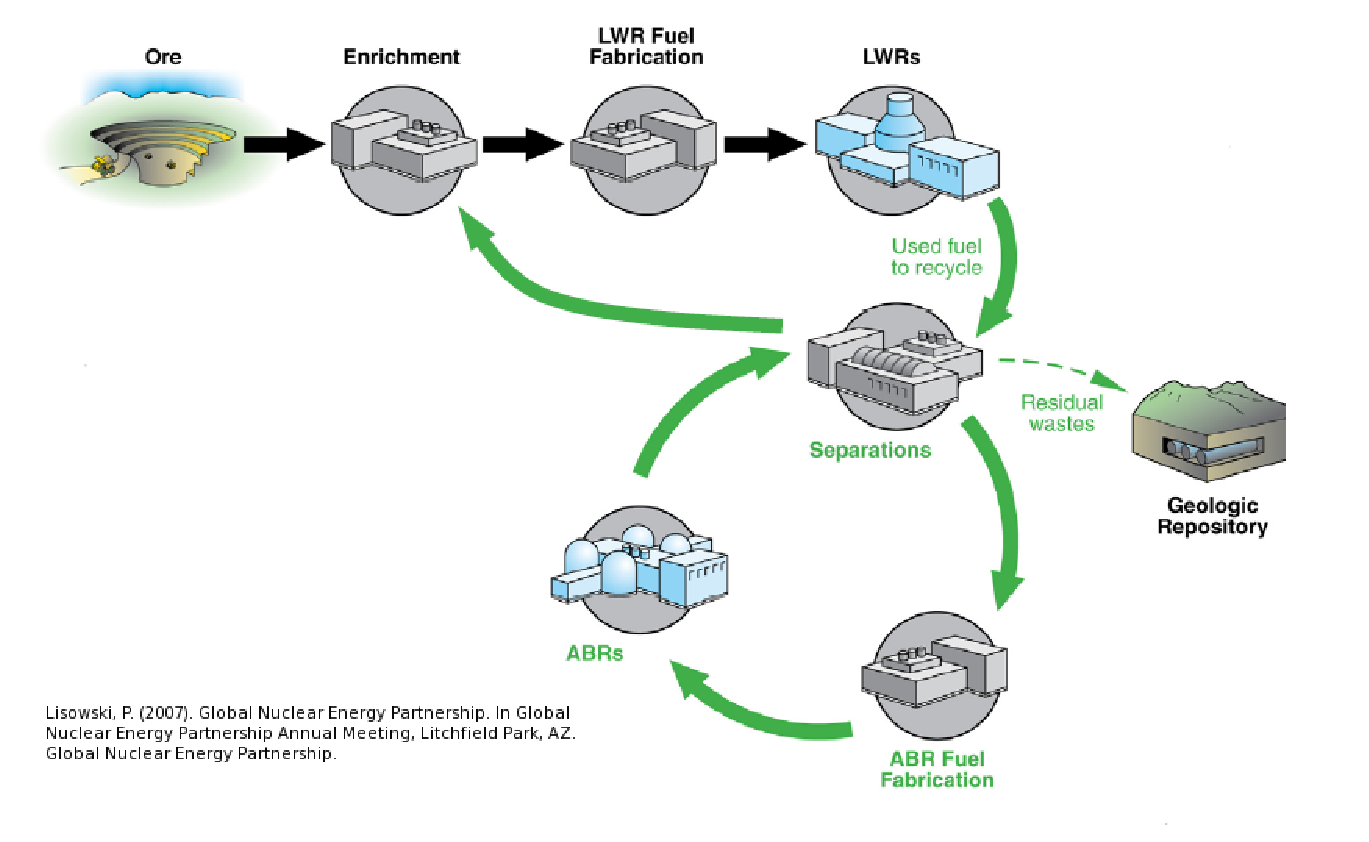
\includegraphics[width=0.6\textwidth]{./cyder/images/simulations.eps}
    \end{center}
    \caption{The Cyclus simulator framework provides an environment for fuel 
    cycle analysis.}
    \label{fig:simulations}
  \end{figure}
  %Cyclus Figure
  %Simulation Figure
}
\end{frame}

\subsection{Modular Barrier Components}

\begin{frame}[ctb!]
  \frametitle{Cyder Framework}
  \footnotesize{
The Cyder repository model architecture is intended to modularly permit 
exchange of disposal system Component models (e.g., detailed nuclide transport 
model vs. less detailed) and data (e.g., exchange clay for granite geologic 
data) and accept arbitrary waste stream isotopic compositions.  
  \begin{figure}[htbp!]
    \begin{center}
      \includegraphics[width=0.6\textwidth]{cyder/images/componentLoading.eps}
      \caption{The Cyder architecture modularly permits exchange of models and 
      data. Documentation and source code can be found at katyhuff.github.com/cyder.}
    \end{center}
  \end{figure}
}
\end{frame}

\begin{frame}[ctb!]
  \frametitle{Cyder Framework : Waste Stream Acceptance}
  \footnotesize{
  
To participate in fuel cycle simulation, the repository model must accept arbitrary 
spent fuel and high level waste streams. A waste stream is a material data 
object resulting from the Cyclus simulated fuel cycle.  
  \begin{figure}[htbp!]
    \begin{center}
      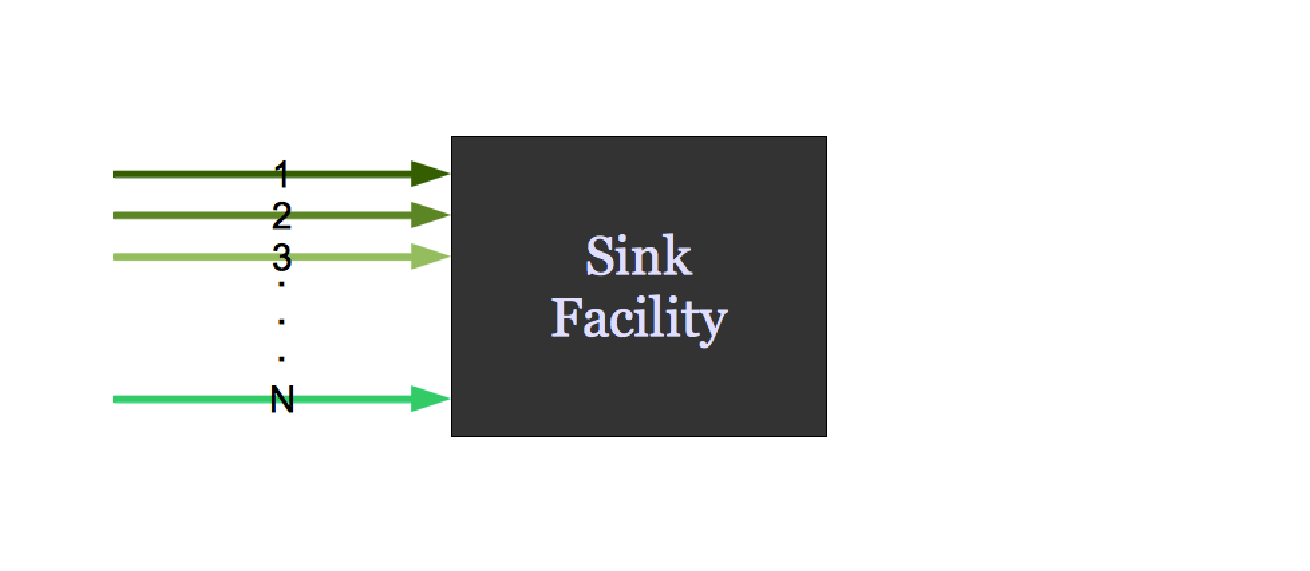
\includegraphics[height=5cm]{./cyder/images/sinkfacility.eps}
    \end{center}
    \caption{ The Cyder Facility dynamically accepts material from the 
    coupled fuel cycle simulation.} 
    \label{fig:sinkfacility}
  \end{figure}
% Sink Facility ?
}
\end{frame}

\begin{frame}[ctb!]
  \frametitle{Cyder Framework : Waste Stream Conditioning}
  \footnotesize{

    \textbf{Waste conditioning} is the process of packing a waste stream into an appropriate 
waste form.  The Cyder model loads discrete waste forms with discrete waste 
stream contaminant vectors as depicted in Figure \ref{fig:ws_conditioning}.
  
\begin{figure}[htbp!]
\begin{center}
\def\svgwidth{.5\textwidth}
\input{./cyder/images/ws_conditioning.eps_tex}
\end{center}
\caption{Waste streams are conditioned into the appropriate waste form 
according to user-specified pairings.}
\label{fig:ws_conditioning}
\end{figure}
}
\end{frame}

\begin{frame}[ctb!]
  \frametitle{Cyder Framework : Waste Form Packaging}
  \footnotesize{

    \textbf{Waste packaging} is the process of placing one or many waste forms into a 
containment package. Once the waste stream has been conditioned into a waste 
form, that waste form Component is loaded into a waste package Component as 
depicted in Figure \ref{fig:wf_packaging}.  

\begin{figure}[htbp!]
\begin{center}
\def\svgwidth{.5\textwidth}
\input{./cyder/images/wf_packaging.eps_tex}
\end{center}
\caption{Waste forms are loaded into the appropriate waste package 
according to user-specified pairings.}
\label{fig:wf_packaging}
\end{figure}
}
\end{frame}

\begin{frame}[ctb!]
  \frametitle{Cyder Framework : Waste Package Emplacement}
  \footnotesize{
  
\begin{columns}[c]
  \column{0.3\textwidth}
  Finally, the waste package is \textbf{emplaced} in a buffer component which 
contains many other waste packages spaced evenly in a grid as in Figure 
\ref{fig:repo_layout}. Repository depth, $\Delta z$, waste package spacing, 
$\Delta x$, and tunnel spacing, $\Delta y$ are user specified.

  \column{0.7\textwidth}

\begin{figure}[htbp!]
\begin{center}
\def\svgwidth{.5\textwidth}
\input{./cyder/images/repo_layout.eps_tex}
\end{center}
\caption{ The grid is defined by the user.  }
\label{fig:repo_layout}
\end{figure}
\end{columns}

}
\end{frame}


\begin{frame}
  \frametitle{Nested Components}
  Each Component has : 
  \begin{itemize}
    \item a Geometry to describe its dimensions and location
    \item a NuclideModel for contaminant transport 
    \item a ThermalModel for heat transport
    \item a Parent Component at its external barrier
    \item one or more Daughter Components at its internal barrier
  \end{itemize}

  Components have other data members such as a Type (WF, WP, BUFFER, FF), a 
  material data table, a start date, etc. 
\end{frame}

\begin{frame}
  \frametitle{Nested Components}
  The NuclideModel in a Component can be interchangeably represented by any of 
  the four nuclide transport models. 
    \begin{itemize}
      \item Degradation Rate Based Failure Model
      \item Mixed Cell with Degradation, Sorption, Solubility Limitation
      \item Lumped Parameter Model
      \item 1D Advection Dispersion Solution
    \end{itemize}
\end{frame}


\section{Hydrologic Models}
\begin{frame}
  \frametitle{Advection Dispersion Equation}
  \footnotesize{
    In a saturated, reducing environment, contaminants are transported by 
    \textbf{dispersion} and \textbf{advection} \cite{schwartz_fundamentals_2003, 
    wang_introduction_1982, van_genuchten_analytical_1982}: 
    \begin{align}
      J &= J_{dis} + J_{adv}\nonumber\\
      &= -\theta(D_{mdis} + \tau D_m)\nabla C + \theta vC\nonumber\\ 
      &= -\theta D\nabla C + \theta vC \nonumber\\ 
      \intertext{which, for uniform flow in $\hat{k}$, is}
      &=\left(-\theta D_{xx} \frac{\partial C}{\partial x}
             \right)\hat{\imath}
             + \left( -\theta D_{yy} \frac{\partial C}{\partial y}
            \right)\hat{\jmath}
            + \left( -\theta D_{zz} \frac{\partial C}{\partial z}
             + \theta v_zC 
            \right)\hat{k},
      \label{unidirflow}
      \intertext{where}
      J_{dis} &= \mbox{ Total Dispersive Mass Flux }[kg/m^2/s]\nonumber\\
      J_{adv} &= \mbox{ Advective Mass Flux }[kg/m^2/s]\nonumber\\
      \tau &= \mbox{ Toruosity }[-] \nonumber\\
      \theta &= \mbox{ Porosity }[\%] \nonumber\\
      D_m &= \mbox{ Molecular diffusion coefficient }[m^2/s]\nonumber\\
      D_{mdis} &= \mbox{ Coefficient of mechanical dispersivity}[m^2/s]\nonumber\\
      D &= \mbox{ Effective Dispersion Coefficient }[m^2/s]\nonumber\\
      C &= \mbox{ Concentration }[kg/m^3]\nonumber\\
      v &= \mbox{ Fluid Velocity in the medium }[m/s].\nonumber
    \end{align}
    }

\end{frame}

\begin{frame}
  \frametitle{Sorption and Solubility}
  \footnotesize{
  In addition to engineered barriers, their movement is constrained by 
  the solubility limit, 
    \begin{align}
      m_i &\leq V_w C_{sol,i},
    \intertext{and sorption,}
      S &=\frac{V_w(C_0 -C)}{m_s}
    \intertext{where}
      m_i &= \mbox{ mass of isotope i in volume }V_w [kg]\nonumber\\ 
      V_w &= \mbox{ volume of the solution }[m^3]\nonumber\\
      C_{sol,i} &= \mbox{ solubility limit, the maximum concentration of i }[kg_m^3]\nonumber\\
      S &= \mbox{ mass sorbed on the surface }[kg/kg]\nonumber\\
      C_0 &= \mbox{ initial concentration in the solution }[kg_m^3]\nonumber\\
      C &= \mbox{ equilibrium concentration in the solution }[kg/m^3]\nonumber\\
      m_s &= \mbox{ sediment mass }[kg].\nonumber
    \end{align}
    The function $S(C)$ is called a sorption isotherm. 
    }
\end{frame}

\begin{frame}
  \frametitle{Component Interfaces}
  \footnotesize{
    For uniform flow in the vertical $\hat{z}$ direction, the governing equation is,

  \begin{align}
    D_x \frac{\partial^2 C}{\partial x^2} +
    D_y \frac{\partial^2 C}{\partial y^2} +
    D_z \frac{\partial^2 C}{\partial z^2} +
    v_z \frac{\partial C}{\partial z}  = R_f \frac{\partial C}{\partial t}.  
    \label{unidirflow}
  \end{align}

  \begin{figure}[htp!]
    \begin{center}
      \def\svgwidth{\textwidth}
      \input{cyder/images/flow.eps_tex}
    \end{center}
    \caption{The boundaries between components are robust interfaces defined by 
    Source Term, Dirichlet, Neumann, and Cauchy boundary conditions.}
    \label{fig:flow}
  \end{figure}
  }
\end{frame}

\begin{frame}
  \frametitle{Boundary Conditions}
  \footnotesize{
    \textbf{First, specified-head or Dirichlet type} boundary conditions define a specified species 
    concentration
      \begin{align}
      C(\vec{r},t) = C_0(\vec{r},t)\hspace{1mm}\mbox{ for } \vec{r} \in 
      \Gamma.
      \intertext{where}
      \vec{r} &= \mbox{ position vector }\nonumber\\
      \Gamma &= \mbox{ domain boundary }\nonumber\\
    \end{align}  
    
    \textbf{Second, specified-flow, or Neumann type} boundary conditions describe a full set of 
    concentration gradients 
   \begin{align}
      \frac{\partial C(\vec{r},t)}{\partial r} &= \theta D\vec{J}(t) 
      \hspace{1mm}\mbox{ for } \vec{r} \in \Gamma.
    \end{align}    
    
    \textbf{Third, head-dependent, or Cauchy type}, defines a solute 
    flux along the boundary,
      \begin{align}
      -D\frac{\partial C}{\partial z} + v_zC &= v_zC(\vec{r},t) 
      \hspace{1mm}\mbox{ for }\vec{r} \in \Gamma.
    \end{align}    
  }
\end{frame}

\begin{frame}
\frametitle{Implicit Timestepping}
\footnotesize{Each Component passes some information radially outward to the nested 
Component immediately containing it and some information radially 
inward to the nested Component it contains. 

Mass distribution in Component 0 at time $t_n$ is found from the inner boundary 
condition at time $t_n$ and the outer boundary condition at $t_{n-1}$. Outer 
boundary conditions are solved for numerically at $t_n$.
For each timestep :

\begin{align}
  BC(i, r_o, c_1, t_n) &= f( BC(i, r_i, c_0, t_n), BC(i, r_o, c_1, t_{n-1}) )
  \intertext{where}
  BC  &= \mbox{boundary condition }\nonumber\\
  i &= \mbox{the isotope }\nonumber\\
  r_i &= \mbox{the inner boundary radius } [m]\nonumber\\
  r_o &= \mbox{the outer boundary radius } [m]\nonumber\\
  c_0 &= \mbox{the innermost Component}\nonumber\\
  c_1 &= \mbox{the Component that contains c}_0\nonumber\\
  f &= \mbox{functional form of the contaminant transport algorithm}\nonumber\\
  t_n &= \mbox{timestep n.}\nonumber
\end{align}
}
\end{frame}

\begin{frame}
  \frametitle{Nested Components}
  Each component represents a 
  \begin{itemize}
    \item Waste Form
    \item Waste Package
    \item Buffer
    \item or Far Field (geologic medium).
  \end{itemize}
\end{frame}


\begin{frame}
  \frametitle{Nested Components}
  Each Component has : 
  \begin{itemize}
    \item a Geometry to describe its dimensions and location
    \item a NuclideModel for contaminant transport 
    \item a ThermalModel for heat transport
    \item a Parent Component at its external barrier
    \item one or more Daughter Components at its internal barrier
  \end{itemize}

  Components have other data members such as a Type (WF, WP, BUFFER, FF), a 
  material data table, a start date, etc. 
\end{frame}

\begin{frame}
  The NuclideModel in a Component can be interchangeably represented by any of 
  the four nuclide transport models. 
    \begin{itemize}
      \item Degradation Rate Based Failure Model
      \item Mixed Cell with Degradation, Sorption, Solubility Limitation
      \item Lumped Parameter Model
      \item 1D Advection Dispersion Solution
    \end{itemize}
\end{frame}

\subsection{Degradation Rate With Congruent Release}
\begin{frame}
  \frametitle{Radionuclide Transport: Rate Based Congruent Release}
  \footnotesize{
  Contaminants are released congruently with degradation of the component.

  That is, for a rate of $\epsilon [\%]$ per year, where the initial condition is some 
  contained mass, $m_0$, the boundary conditions supplied to external components 
  at the outer boundary $r_{bc}$are :

  \begin{align}
    \intertext{Source Term}
    \dot{m} &= \epsilon m_0
    \intertext{Dirichlet}
    C(r_{bc}) &= \dot{m}/V_w 
    \intertext{Neumann}
    \frac{\partial C}{\partial r} &= ( \dot{m}/V_w - C_{ext} )/(r_{ext} - r_{in})
    \intertext{Cauchy}
    -D \frac{\partial C}{\partial x}\big|_{x=x_{bc}} + v_xc &= vC(x_{bc}) 
  \end{align}
  }
\end{frame}

\begin{frame}
  \frametitle{Radionuclide Transport: Rate Based Congruent Release}
  \footnotesize{
The implemented model incorporates the source term made available on the inner boundary into its available mass and defines the resulting boundary conditions at the outer boundary as solely a function of the degradation rate of that component.

This results in the following expression for the mass transfer, 
$m_{ij}(t)$, from cell $i$ to cell $j$ at time $t$ :

\begin{align}
  \dot{m}_{ij}(t) &= f_i(\cdots)m_i(t)
  \label{deg_rate_source_cont}
  \intertext{where}
  \dot{m}_{ij} &= \mbox{ the rate of mass transfer from i to j 
  }[kg/s]\nonumber\\
  f_i &= \mbox{ fractional degradation rate in cell i }[1/s] \nonumber\\
  m_i &= \mbox{ mass in cell i }[kg] \nonumber\\
  t &= \mbox{ time  }[s].\nonumber
\end{align}
}
\end{frame}


\begin{frame}
  \frametitle{Radionuclide Transport: Rate Based Congruent Release}
  \footnotesize{
For a situation as in Cyder and Cyclus, with discrete timesteps, the timesteps 
are 
assumed to be small enough to assume a constant rate $m_{ij}$ over the course of 
the timestep. The mass transferred between discrete times $t_{n-1}$ and $t_n$ is 
thus a simple linear function of the transfer rate in 
\eqref{deg_rate_source_cont}, 

\begin{align}
  m_{ij}^n &= \int_{t_{n-1}}^{t_n}\dot{m}_{ij}(t')dt' \nonumber\\
           &= f_i(\cdots)m_i^{n-1}\left(t_n - t_{n-1}\right).
           \label{deg_rate_source_discrete}
\end{align}
}
\end{frame}


\subsection{Mixed Cell With Sorption and Solubility}
\begin{frame}
  \frametitle{Radionuclide Transport: Mixed Cell}
  % Waste Form
  \begin{figure}[h!]
    \begin{center}
      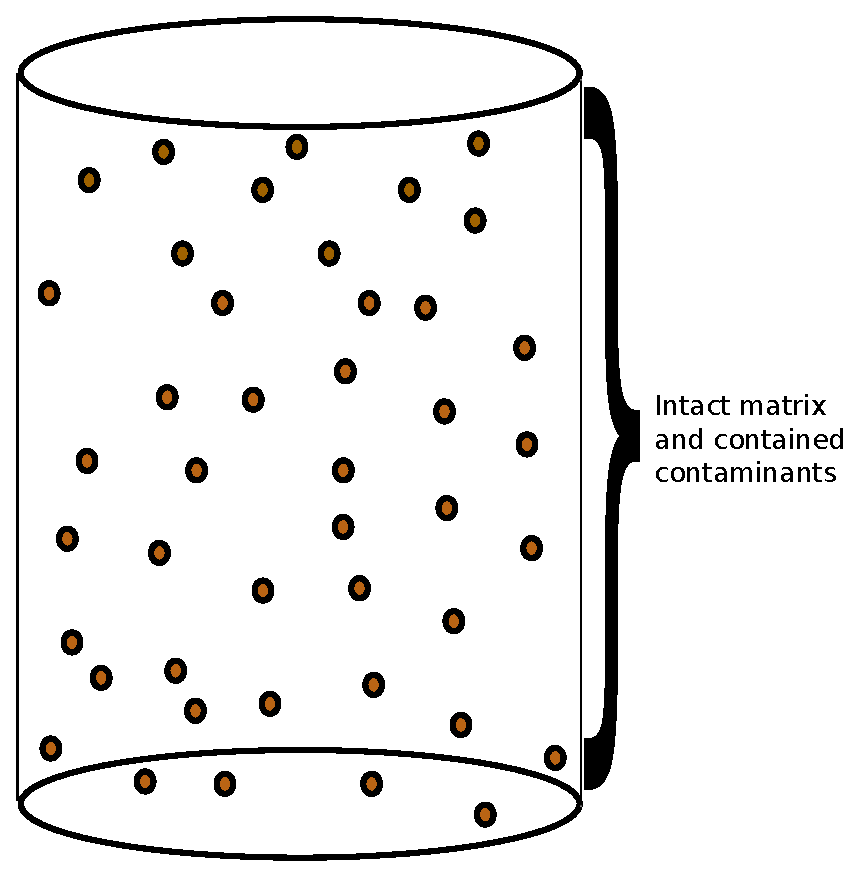
\includegraphics[height=.6\textwidth]{cyder/images/mixed_cell_whole.eps}
    \end{center}
  \end{figure}
\end{frame}

\begin{frame}[ctb!]
  \frametitle{Radionuclide Transport: Mixed Cell}
  % Waste Form
  \begin{figure}[h!]
    \begin{center}
      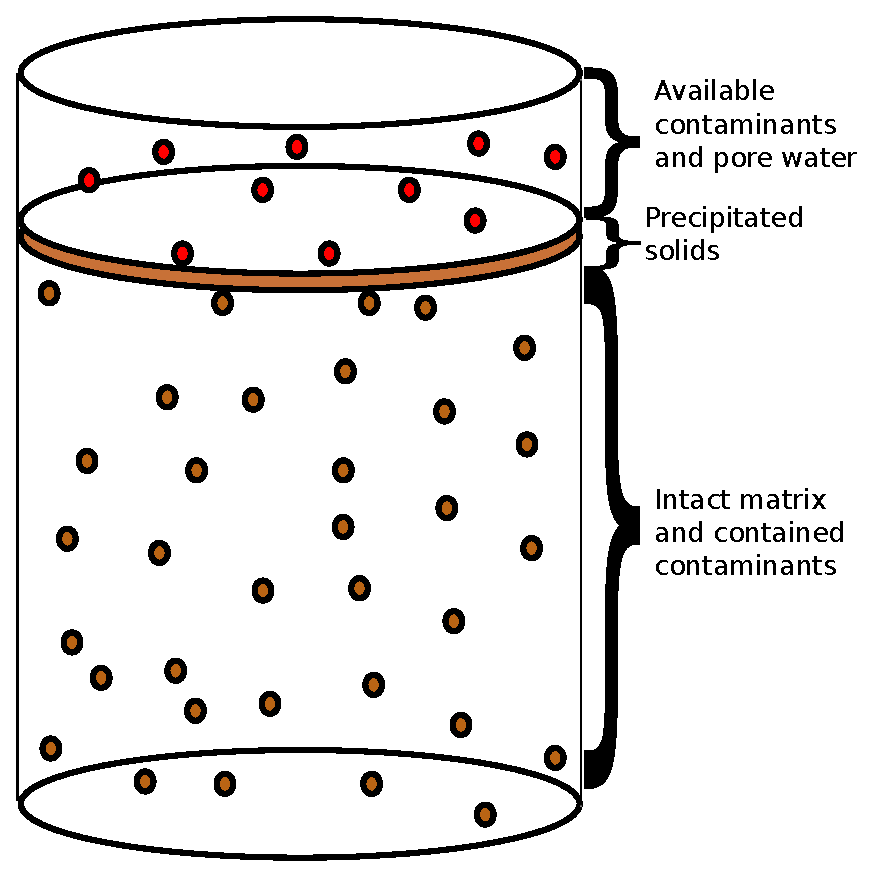
\includegraphics[height=.6\textwidth]{cyder/images/mixed_cell_degraded.eps}
    \end{center}
  \end{figure}
\end{frame}


\subsection{Lumped Parameter Transport}
\begin{frame}
  \frametitle{Radionuclide Transport: Lumped Parameter Transport Model}
\footnotesize{
\begin{figure}[htbp!]
  \begin{center}
    \def\svgwidth{\textwidth}
    \input{cyder/images/lumpedseries.eps_tex}
  \end{center}
  \caption{ The method by which each lumped parameter component is modeled is
according to a relationship between the incoming concentration, $C_{in}(t)$,
and the outgoing concentration, $C_{out}(t)$.}
  \label{fig:lumpedseries}
\end{figure}

\begin{align}
  C_{out}(t) &= \int_{-\infty}^t C_{in}(t')g(t-t')e^{-\lambda(t-t')}dt'
  \label{lumped1}
  \intertext{equivalently}
  C_{out}(t) &= \int_0^\infty C_{in}(t-t')g(t')e^{-\lambda t'}dt'
  \label{lumped2}
  \intertext{where}
  t'  &= \mbox{ time of entry }[s]\nonumber\\
  t-t'  &= \mbox{ transit time }[s]\nonumber\\
  g(t-t')  &= \mbox{ response function, a.k.a. transit time 
  distribution}[-]\nonumber]\\
  \lambda &= \mbox{ radioactive decay constant, 1 to neglect}[s^{-1}].\nonumber
\end{align}
}
\end{frame}

\begin{frame}
  \frametitle{Radionuclide Transport: Lumped Parameter Transport Model}
\footnotesize{
Selection of the response function is usually based on experimental tracer 
results in the medium at hand. However, some functions used commonly in chemical 
engineering applications \cite{maloszewski_lumped_1996} include the Piston Flow Model (PFM), 
\begin{align}
  g(t') &= \delta{(t'-t_t))}
  \intertext{ the Exponential Model (EM) }
  g(t') &= \frac{1}{t_t}e^{-\frac{t'}{t_t}}
  \intertext{ and the Dispersion Model (DM), }
  g(t') &= \left( \frac{\texttt{Pe }t_t}{4\pi t'} \right)^{\frac{1}{2}}
  \frac{1}{t'}e^{- \frac{\texttt{Pe }t_t\left( 1- \frac{t'}{t_t}  \right)^2} 
  {4t'}}, \intertext{where}
  \texttt{Pe }  &= \mbox{ Peclet number for mass diffusion }[-]\nonumber\\
  t_t  &= \mbox{ mean tracer age }[s]\nonumber\\
    &= t_w \mbox{ if there are no stagnant areas }\nonumber\\
  t_w  &= \mbox{ mean residence time of water }[s]\nonumber\\
       &= \frac{V_m}{Q}\nonumber\\
       &= \frac{z}{v_z}\nonumber\\
       &= \frac{z\theta_e}{q}\nonumber
  \intertext{in which}
  V_m  &= \mbox{ mobile water volume }[m^3]\nonumber\\
  Q    &= \mbox{ volumetric flow rate }[m^3/s]\nonumber\\
  z    &= \mbox{ average travel distance in flow direction }[m]\nonumber\\
  v_z  &= \mbox{ mean water velocity}[m/s]\nonumber\\
  q    &= \mbox{ Darcy Flux }[m/s]\nonumber\\
  \theta_e &= \mbox{ effective (connected) porosity }[\%].\nonumber
\end{align}
}
\end{frame}

\begin{frame}
  \frametitle{Radionuclide Transport: Lumped Parameter Transport Model}
\footnotesize{
The latter of these, the Dispersion Model satisfies the one dimensional 
advection-dispersion equation, and is therefore the most physically relevant for 
this application. The solutions to these for constant concentration at the 
source boundary are given in \cite{maloszewski_lumped_1996}, 
\begin{align}
  C(t) &=\begin{cases}
    PFM & C_0e^{-\lambda t_t}\\
    EM  & \frac{C_0}{1+\lambda t_t}\\
    DM & C_0e^{\frac{\texttt{Pe}}{2}\left(1-\sqrt{1+\frac{4\lambda 
    t_t}{\texttt{Pe}}}\right)}.
  \end{cases}
  \label{lumpedsolns}
\end{align}
}
\end{frame}


\begin{frame}
  \frametitle{Radionuclide Transport: Lumped Parameter Transport Model}
\footnotesize{
Selection of the response function is usually based on experimental tracer 
results. Canonical forms include :
\begin{align}
  \mbox{the Piston Flow Model (PFM), } g(t') &= \delta{(t'-t_t))}\\
  \mbox{ the Exponential Model (EM), } g(t') &= 
  \frac{1}{t_t}e^{-\frac{t'}{t_t}}\\
  \mbox{ and the Dispersion Model (DM), } g(t') &= \frac{\left[ \left( \frac{t\pi t'}{t_t Pe} \right) 
  (\frac{1}{t'})e^{- \left( 1- \frac{t'}{t_t}  \right)^2} 
  \right]}{\frac{4t'}{t_tPe}}, 
  \intertext{where}
  Pe  &= \mbox{ Peclet number }[-]\nonumber\\
  t_t  &= \mbox{ mean tracer age }[s]\nonumber\\
    &= t_w \mbox{ if there are no stagnant areas}\nonumber\\
  t_w  &= \mbox{ mean residence time of water}[s].\nonumber\\
\intertext{The solutions to these for constant concentration at the source 
boundary give}
  C(t) &=\begin{cases}
    PFM & C_0e^{-\lambda t_t}\\
    EM  & \frac{C_0}{1+\lambda t_t}\\
    DM  & \frac{C_0e^{Pe\sqrt{\left( 1-(1+\frac{4\lambda t_t}{Pe})\right)}}}{2}\\
  \end{cases}
  \label{lumpedsolns}
\end{align}
}
\end{frame}

\subsection{1D Semi-Infinite, Cauchy B.C.}
\begin{frame}
  \frametitle{Radionuclide Transport: 1D Semi-Infinite, Cauchy B.C.}
  \footnotesize{
\begin{figure}[htbp!]
  \begin{center}
    \def\svgwidth{.5\textwidth}
    \input{cyder/images/1dinf.eps_tex}
  \end{center}
  \caption{A one dimensional, semi-infinite model, unidirectional flow,
  solution with Cauchy and Neumann boundary conditions}
  \label{fig:1dinf}
\end{figure}
The solution is given (Leij et al., \cite{leij_analytical_1991})  for the
boundary conditions :

For the boundary conditions, 
\begin{align}
  -D \frac{\partial C}{\partial z}\big|_{z=0} + v_zc &= \begin{cases}
    v_zC_0  &  \left( 0<t<t_0 \right)\\
    0  &  \left( t>t_0 \right)\\
  \end{cases},\\
  \frac{\partial C}{\partial z}\big|_{z=\infty} &= 0
  \intertext{and the initial condition,}
  C(z,0) &= C_i.
  \label{1dinfBC}
\end{align}
}
\end{frame}

\begin{frame}
\frametitle{Radionuclide Transport: 1D Semi-Infinite, Cauchy B.C.}
\footnotesize{
The solution is given (Leij et al., \cite{leij_analytical_1991})  as :
\begin{align}
  C(z,t) &= 
  \frac{C_0}{4}\int_0^t\frac{v}{R}\Lambda_3(\tau)\Gamma_2(\tau)d\tau + 
  \frac{\lambda}{2R}\int_0^t\Lambda_4(\tau)
  \intertext{which, for no $\lambda$ first order production becomes}
  &= \frac{C_0}{4}\int_0^t\frac{v}{R}\Lambda_3(\tau)\Gamma_2(\tau)d\tau
  \intertext{where}
  R &= \mbox{Retardation factor }[-].
\end{align}
}
\end{frame}

\begin{frame}
\frametitle{Radionuclide Transport: 1D Semi-Infinite, Cauchy B.C.}
\footnotesize{
For the vertical flow coordinate system, $\Lambda_3$ and $\Gamma_2$ are defined 
as
\begin{align}
  \Lambda_3(\tau) &= e^{-\frac{\mu\tau}{R}}\Bigg[\sqrt{\frac{R}{\pi D_z\tau}}e^{-\frac{(Rz-v\tau)^2}{4RD_z\tau}} - 
    \frac{v}{2D_z}e^\frac{vz}{D_z}\erfc{\frac{Rz+v\tau}{\sqrt{4RD_z\tau}}}\Bigg]
    \label{Lambda_3}
  \intertext{and}
  \Gamma_2(\tau) &= 
      \Bigg[ \erfc{\frac{x-a}{\sqrt{\frac{4D_x\tau}{R}}} } - 
             \erfc{\frac{x+a}{\sqrt{\frac{4D_x\tau}{R}}} } \Bigg]
      \Bigg[ \erfc{\frac{y-b}{\sqrt{\frac{4D_y\tau}{R}}} } -
             \erfc{\frac{y+b}{\sqrt{\frac{4D_y\tau}{R}}} } \Bigg]. 
      \label{Gamma_2}
\end{align}
}
\end{frame}

\begin{frame}
\frametitle{Radionuclide Transport: 1D Semi-Infinite, Cauchy B.C.}
\footnotesize{
We make a few simplifying one dimensional assumptions. First, that the diffusion 
coefficient of the medium is the same in the $\hat{x}$ and $\hat{y}$ directions 
such that $D_x=D_y$. Also, we take the concentration around the origin for a 
unit surface area, so $x=y=0$ and $a=b=1$. Thus, $\Gamma_2$ from equation \eqref{Gamma_2} becomes
\begin{align}
  \Gamma_2(\tau) = 2\left(\erfc{\frac{1}{\sqrt{\frac{4D_{xy}\tau}{R}}} 
}^2\right).
\end{align}
}
\end{frame}

\begin{frame}
\frametitle{Radionuclide Transport: 1D Semi-Infinite, Cauchy B.C.}
\footnotesize{
Another simplification is that, in Cyclus, radioactive decay is handled external 
to the components, so $\mu$, the constant of decay in equation \eqref{Lambda_3}, 
goes to zero. Thus, 

\begin{align}
  C(z,t)&= \frac{C_0}{2}\int_0^t\frac{v}{R}
  \Bigg[\sqrt{\frac{R}{\pi D_z\tau}}e^{-\frac{(Rz-v\tau)^2}{4RD_z\tau}} -
    \frac{v}{2D_z}e^\frac{vz}{D_z}\erfc{\frac{Rz+v\tau}{\sqrt{4RD_z\tau}}}\Bigg]
    \erfc{\frac{1}{\sqrt{\frac{4D_{xy}\tau}{R}}} }^2
  d\tau .
  \label{simple_leij}
\end{align}
}
\end{frame}

\section{Demonstration}
\begin{frame}
  \frametitle{Degradation Rate Base Case I}
  Base Case I : If the degradation rate of the waste form is 0, then no nuclides should be 
  transported out of it, irrespective of the degradation rates of other 
  barriers. 

  \begin{figure}[htbp!]
    \begin{center}
      \includegraphics[width=\textwidth]{cyder/images/stub_0deg_comp_table.eps}
    \end{center}
  \end{figure}
\end{frame}

\begin{frame}
  \frametitle{Degradation Rate Base Case I}
  Base Case I : If the degradation rate of the waste form is 0, then no nuclides should be 
  transported out of it, irrespective of the degradation rates of other 
  barriers. 

  \begin{figure}[htbp!]
    \begin{center}
      \includegraphics[width=\textwidth]{cyder/images/stub_0deg_cont_table.eps}
      \caption{A number of base cases were run to investigate the performance of 
      the nuclide transport models.}
    \end{center}
  \end{figure}
\end{frame}

\begin{frame}
  \frametitle{Degradation Rate Base Case I}
  Base Case I : If the degradation rate of the waste form is 0, then no nuclides should be 
  transported out of it, irrespective of the degradation rates of other 
  barriers. 

  \begin{figure}[htbp!]
    \begin{center}
      \includegraphics[width=.5\textwidth]{cyder/images/0deg_comp6.eps}
      \includegraphics[width=.5\textwidth]{cyder/images/0deg_comp7.eps}
    \end{center}
  \end{figure}
\end{frame}

\begin{frame}
  \frametitle{Degradation Rate Base Case I}
  Base Case I : If the degradation rate of the waste form is 0, then no nuclides should be 
  transported out of it, irrespective of the degradation rates of other 
  barriers. 

  \begin{figure}[htbp!]
    \begin{center}
      \includegraphics[width=.5\textwidth]{cyder/images/0deg_comp8.eps}
      \includegraphics[width=.5\textwidth]{cyder/images/0deg_comp9.eps}
    \end{center}
  \end{figure}
\end{frame}

\begin{frame}
  \frametitle{Degradation Rate Base Case I}
  Base Case I : If the degradation rate of the waste form is 0, then no nuclides should be 
  transported out of it, irrespective of the degradation rates of other 
  barriers. 

  \begin{figure}[htbp!]
    \begin{center}
      \includegraphics[width=.2\textwidth]{cyder/images/0deg_comp6.eps}
      \includegraphics[width=.2\textwidth]{cyder/images/0deg_comp8.eps}
      \includegraphics[width=.2\textwidth]{cyder/images/0deg_comp10.eps}
      \includegraphics[width=.2\textwidth]{cyder/images/0deg_comp12.eps}
      \includegraphics[width=.2\textwidth]{cyder/images/0deg_comp14.eps}
    \end{center}
  \end{figure}
\end{frame}

\begin{frame}
  \frametitle{Degradation Rate Base Case I}
  Base Case I : If the degradation rate of the waste form is 0, then no nuclides should be 
  transported out of it, irrespective of the degradation rates of other 
  barriers. 

  \begin{figure}[htbp!]
    \begin{center}
      \includegraphics[width=.7\textwidth]{cyder/images/0deg.eps}
    \end{center}
  \end{figure}
\end{frame}


\begin{frame}[ctb]
\frametitle{Sensitivity Analysis with the Clay Generic Disposal System Model}

Recall : Abstraction process uses results from more detailed models to improve 
speed and accuracy of analytical models. In this case, sensitivity analyses were 
conducted using the Used Fuel Disposition Campaign's Clay Generic Disposal System 
Model \cite{huff_key_2012} in order to inform the analytic models just discussed.

\begin{table}[ht!]
\centering
\footnotesize{
\begin{tabular}{|l|l|l|r|r|}
\multicolumn{5}{c}{\textbf{Simulation Cases}}\\
\hline
\textbf{Case} & \textbf{Parameter} & \textbf{Units} & \textbf{Min. Value} & \textbf{Max. Value}\\
\hline
I     & $D_{eff}$    & $[m^2\cdot s^{-1}]$       & $10^{-8}$    &  $10^{-5}$ \\
      & Inventory              & [MTHM]         & $10^{-4}$    &  $10^1$ \\
\hline
II    & $V_{adv, y}$ & $[m \cdot yr^{-1}]$       & $6.31\times10^{-8}$  &  $6.31\times10^{-4}$ \\
      & $D_{eff}$    & $[m^2\cdot s^{-1}]$       & $10^{-8}$    &  $10^{-5}$ \\
\hline
III   & $S_i$        & $[mol\cdot m^{-3}]$       & $(1\times10^{-9})\langle S_i\rangle $    &  $(5\times10^{10})\langle S_i\rangle $ \\
\hline
IV    & $K_{d,i}$    & $[m^3\cdot kg^{-1}]$       & $(1\times10^{-9})\langle K_{d,i}\rangle $    &  $(5\times10^{10})\langle K_{d,i}\rangle $ \\
\hline
V     & $R_{WFDeg.}$           & $[yr^{-1}]$       & $10^{-9}$    &  $10^{-2}$ \\
      & Inventory              & [MTHM]         & $10^{-4}$    &  $10^1$ \\
\hline 
VI    & $t_{WPFail}$        & $[yr]$         & $10^3$    &  $10^7$ \\
      & $D_{eff}$           & $[m^2\cdot s^{-1}]$       & $10^{-8}$    &  $10^{-5}$ \\
\hline
\end{tabular}
\caption{Each dual and single parameter simulation case had 40 simulation 
groups of 100 realizations each.}
\label{tab:Cases}
}
\end{table}



\end{frame}


\begin{frame}[ctb]
\frametitle{Solubility Sensitivity}
\begin{figure}[ht]
  \centering
  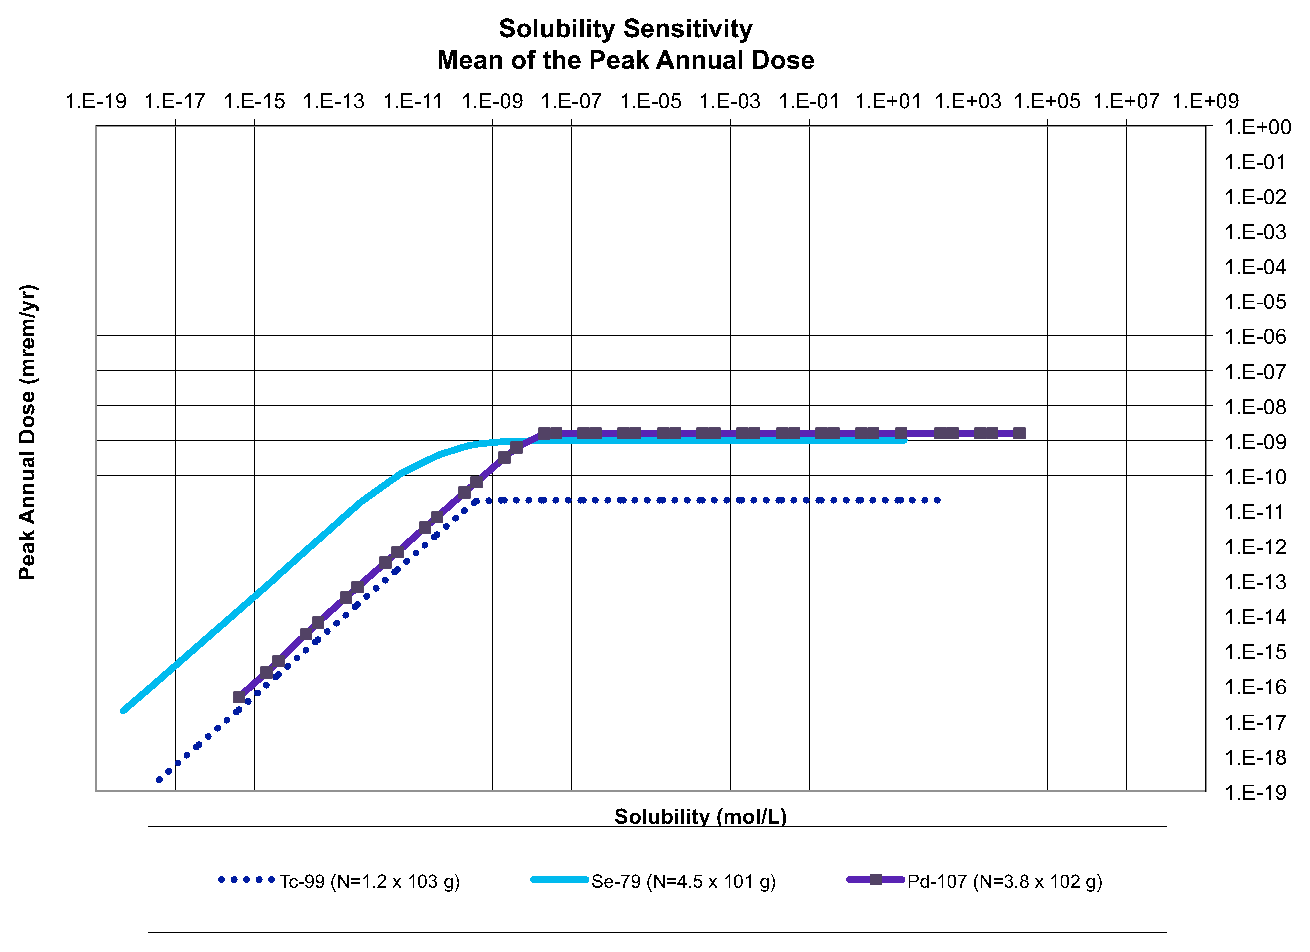
\includegraphics[height=60mm]{cyder/images/Solubility_Summary.eps}
  \caption{Generated with the Used Fuel Disposition Campaign's Generic Disposal 
  System Model for Clay, this graph demonstrates solubility limit sensitivity. 
  The peak annual dose due to an inventory, $N$, of each isotope.}
  \label{fig:SolSum}
\end{figure}
\end{frame}

\begin{frame}[ctb]
\frametitle{Retardation Sensitivity}
\begin{figure}[ht]
  \centering
  \includegraphics[height=60mm]{cyder/images/Partitioning_Summary.eps}
  \caption{Generated with the Used Fuel Disposition Campaign's Generic Disposal 
  System Model for Clay, this graph demonstrates $K_d$ sensitivity. 
  The peak annual dose due to an inventory, $N$, of each isotope.}
  \label{fig:KdSum}
\end{figure}
\end{frame}



\begin{frame}[ctb!]
  \frametitle{Summary}
  Completed infrastructure includes :
  \begin{itemize}
  \item[$\checkmark$] Generic Repository infrastructure 
  \item[$\checkmark$] Modular component loading
  \item[$\checkmark$] Gridded geometry and placement
  \item[$\checkmark$] A Degradation Rate Based Model
  \item[$\checkmark$] A Mixed Cell Model with Sorption and Solubility Limitation
  \item[$\checkmark$] A Lumped Parameter Model
  \item[$\checkmark$] A Detailed 1D Advection Dispersion Model
  \item[$\checkmark$] Databased, plottable results
  \item[$\checkmark$] Fundamental base cases demonstrate nuclide transport 
  \item[$\checkmark$] Agreement with analytic solutions in a suite of unit tests
  \end{itemize}
  Further testing, abstraction, and sensitivity analyses include:
  \begin{itemize}
  \item[$\square$] Robustly check for mass conservation for all models 
  \item[$\square$] Run longer term sensitivity analyses on sorption and solubility 
  \item[$\square$] Robust comparison with component-level GoldSim demonstration 
  \end{itemize}

\end{frame}




\section*{ACKNOWLEDGEMENTS}
This work is supported by the U.S. Department of Energy, Basic Energy Sciences, 
Office of Nuclear Energy, under contract \# DE-AC02-06CH11357.

%%--------------------------------%%
%%--------------------------------%%
\begin{frame}[allowframebreaks]
  \frametitle{References}
  \bibliographystyle{plain}
  {\footnotesize \bibliography{pres} }

\end{frame}

%%--------------------------------%%





\end{document}




